% LaTeX Article Template - customizing page format
%
% LaTeX document uses 10-point fonts by default.  To use
% 11-point or 12-point fonts, use \documentclass[11pt]{article}
% or \documentclass[12pt]{article}.
\documentclass{article}

% Set left margin - The default is 1 inch, so the following 
% command sets a 1.25-inch left margin.
\setlength{\oddsidemargin}{0.25in}

% Set width of the text - What is left will be the right margin.
% In this case, right margin is 8.5in - 1.25in - 6in = 1.25in.
\setlength{\textwidth}{6in}

% Set top margin - The default is 1 inch, so the following 
% command sets a 0.75-inch top margin.
\setlength{\topmargin}{-0.25in}

% Set height of the text - What is left will be the bottom margin.
% In this case, bottom margin is 11in - 0.75in - 9.5in = 0.75in
\setlength{\textheight}{8in}
\usepackage{fancyhdr}
\usepackage{float}
\usepackage{mathtools}
\usepackage{amsmath}
\usepackage{amssymb}
\usepackage{graphicx}
\graphicspath{ {./} }

\setlength{\parskip}{5pt} 
\pagestyle{fancyplain}
% Set the beginning of a LaTeX document
\begin{document}

\lhead{Drew Remmenga MATH 335}
\rhead{HW \#7}
%\lhead{Independent Study}
%\rhead{R Lab}

\begin{enumerate}
\item
	\begin{enumerate}
	\item
	Since we are looking at a mixed distribution it is non-normal. It has a scew to it caused by the quotient which is still normal and the numerator which is also normal. That mixed distribution produces scew which isn't represented by a normal distribution well. 
	\item
	\begin{equation*}
	\begin{split}
	x &= rnorm(5000, 50, 10) \\
	y &= rnorm(5000, 20, 2) \\
	r &= (x*y)/(x+y) \\
	\end{split}
	\end{equation*}
	\item
	\begin{equation*}
	\begin{split}
	prob &= length(r[14 < r \& r < 16])/length(r) \\
	prob &=
	\end{split}
	\end{equation*}
	\item
	\begin{equation*}
	\begin{split}
	prob &= .4652
	\end{split}
	\end{equation*}
	\item
	\begin{equation*}
	\begin{split}
	\bar{X} &= 14.14264 \\
	\hat{\sigma} &= 1.321788
	\end{split}
	\end{equation*}
	\item
	\begin{equation*}
	\begin{split}
	quantile(r,.025)  &= 11.53732 \\
	quantile(r, .975) & = 16.71033 \\
	[11.53732, 16.71033] 
	\end{split}
	\end{equation*}
	\end{enumerate}
\item
	I took one of my mood scales, in particular suicidal ideation rated on scale out of ten every day. \\
	s = c(4,3,4,6,4,7,3,2,1,6)
\item
	\begin{enumerate}
	\item Boxplot and Histogram
	\begin{figure}[H]
		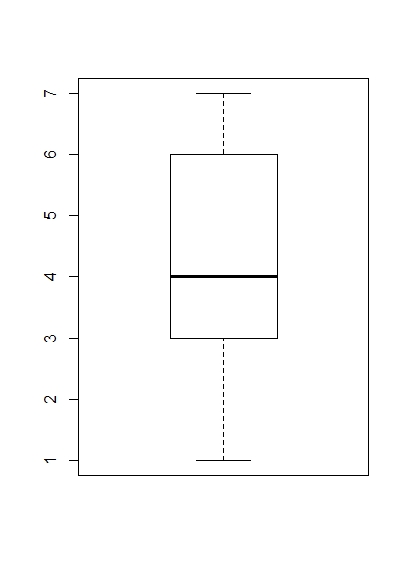
\includegraphics[scale=.45]{boxplotsuicide.png}
	\end{figure}
	\begin{figure}
		\includegraphics[scale = .5]{histsuicide.png}
	\end{figure}
	\item
	\begin{equation*}
	\begin{split}
	ssample& = matrix(rpois(50000, mean(s)),ncol = 10)\\
	x &= apply(ssample,1,sd)\\
	bias &= mean(x) - sd(s)\\
	bias &= .06025199\\
	\end{split}
	\end{equation*}
	\item
	\begin{equation*}
	\begin{split}
	ssample& = matrix(rpois(50000, mean(s)),ncol = 10) \\
	x &= apply(ssample,1,mean)\\
	bias &= mean(x) - mean(s)\\
	bias &= -0.00754\\
	\end{split}
	\end{equation*}
	\item
	\begin{equation*}
	\begin{split}
	quantile(x,.025) &= 2.8 \\
	quantile(x,.975)&= 5.2025 
	\end{split}
	\end{equation*}
	\end{enumerate}
\item
	\begin{enumerate}
	\item
	mean = 5.075086
	sd = 5.37318
		\begin{figure} [H]
		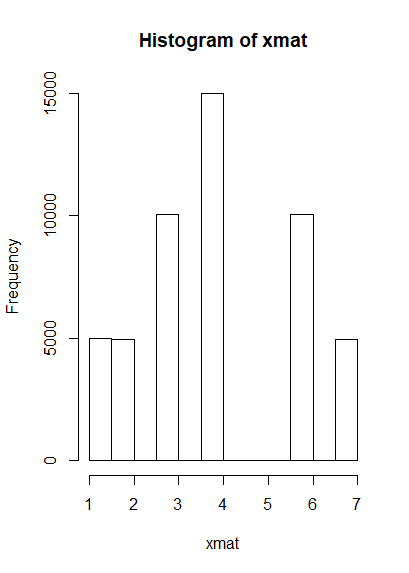
\includegraphics[scale = .5]{histsuicidenon.png}
		\end{figure}
	\item 
	quantile(xmat,.025) = 1.23879
	quantile(xmat,.975) = 6.75321
	\end{enumerate}
\item
	\begin{enumerate}
	\item
	Take $\bar{X}$. Which may be consistent for $\mu$ but could be biased based on the underlying data. The real distribution could be really strange and our sample size is small so consistency doesn't matter a whole lot. 

	\end{enumerate}
\end{enumerate}

\end{document}
